\subsection{Evaluation of Data Transmissions to/from the Android Emulator}
\subsubsection{Android App as client}
\begin{figure}[H]
	\centering
	\begin{subfigure}{.49\textwidth}
		\centering
		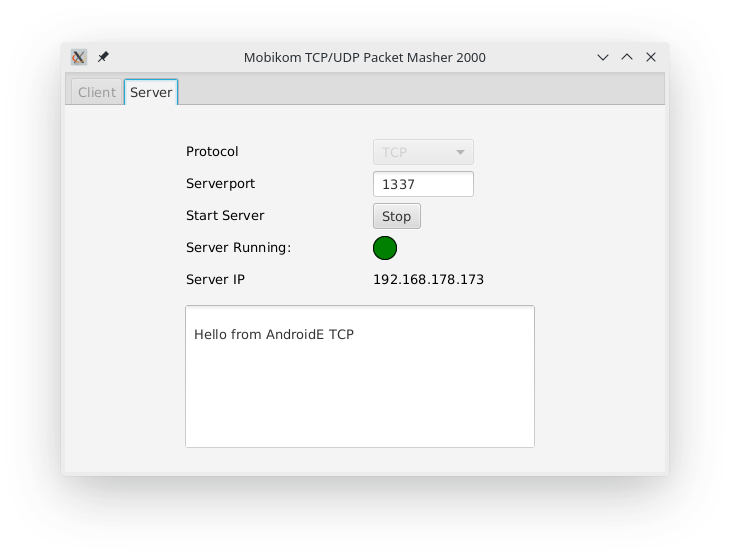
\includegraphics[width=1\linewidth]{images/task3/subtask1/jvmservertcp.png}
		\caption{JVM server using TCP}
		\end{subfigure}
	\begin{subfigure}{.49\textwidth}
		\centering
		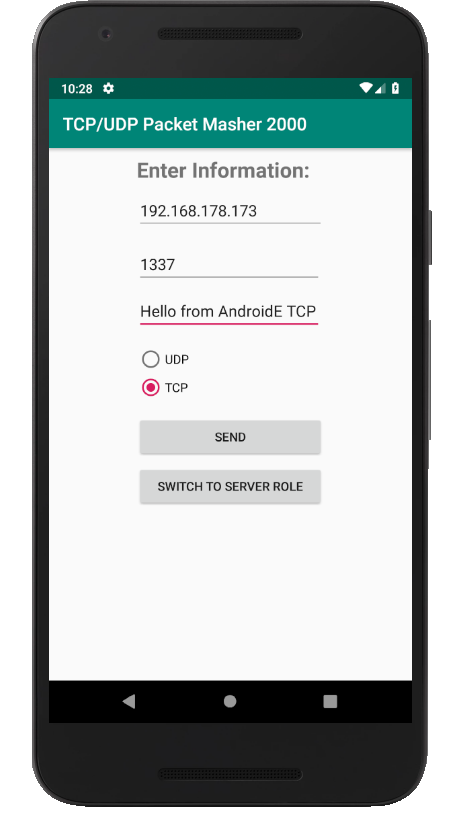
\includegraphics[width=0.74\linewidth]{images/task3/subtask1/androidclienttcp.png}
		\caption{Android client using tcp}
	\end{subfigure}%
	\caption{Android emulator as TCP client}
\end{figure}

\texttt{....sr..communication.Message...........L..messaget..Ljava/lang/String;xpt..Hello from AndroidE TCP} 

\begin{figure}[H]
	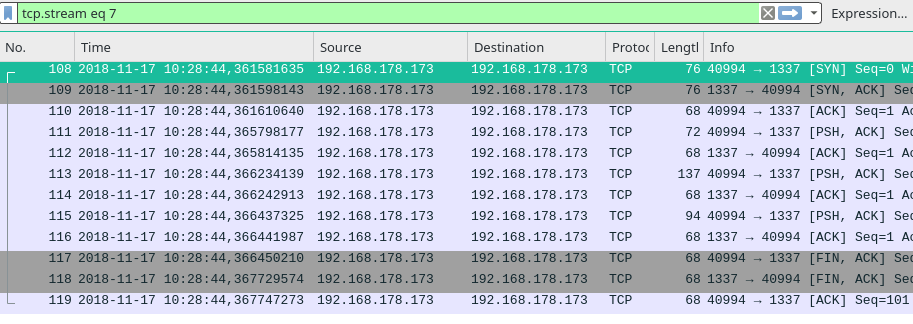
\includegraphics[width=1\linewidth]{images/task3/subtask1/wiresharkTCP.png}
	\caption{Wireshark traces where Android App acts as a TCP client}
\end{figure}

The whole procedure was repeated using the UDP protocol, please find the findings below:\\

\begin{figure}[H]
	\centering
	\begin{subfigure}{.49\textwidth}
		\centering
		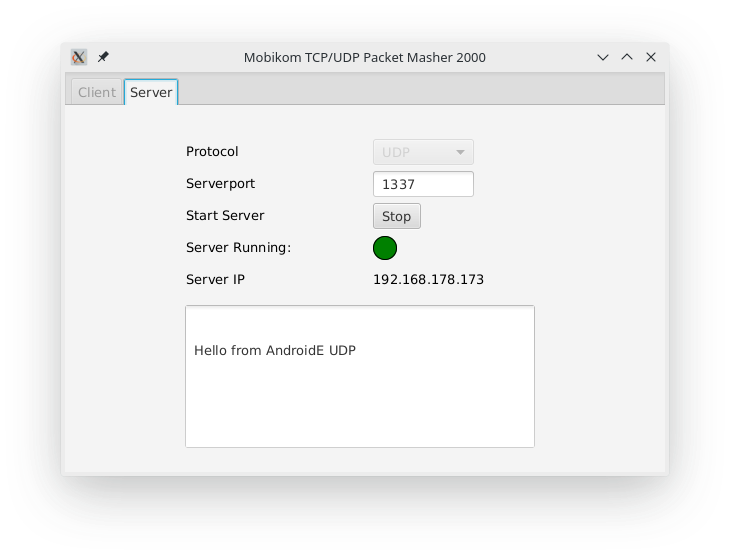
\includegraphics[width=1\linewidth]{images/task3/subtask1/jvmserverudp.png}
		\caption{JVM server using UDP}
	\end{subfigure}
	\begin{subfigure}{.49\textwidth}
		\centering
		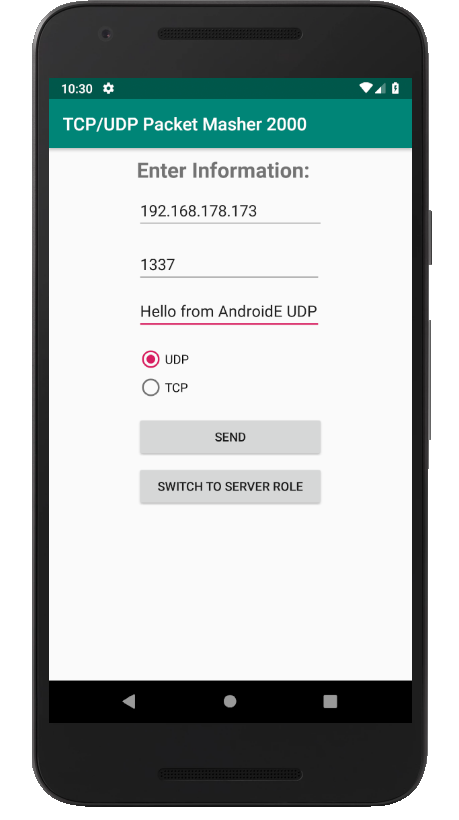
\includegraphics[width=0.74\linewidth]{images/task3/subtask1/androidclientudp.png}
		\caption{Android client using UDP}
	\end{subfigure}%
	\caption{Android emulator as UDP client}
\end{figure}

\texttt{....sr..communication.Message...........L..messaget..Ljava/lang/String;xpt..Hello from AndroidE UDP}
\begin{figure}[H]
	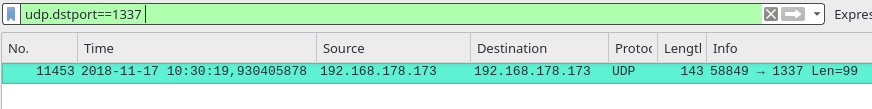
\includegraphics[width=1\linewidth]{images/task3/subtask1/wiresharkUDP.png}
	\caption{Wireshark traces where Android App acts as a UDP client}
\end{figure}

\subsubsection{Android App as server}

The Android Emulator that is shipped with Android Studio puts the virtual device(s) behind a virtual router/firewall, that blocks communication with the host machine by default. In order to test the sending and receiving of TCP/UDP packages, special commands have to be executed allowing the specific flow of packets entering/leaving the virtualized Android instance.\\

The first possibility is to make use of the emulator instance's control console. The following steps are needed: 

\begin{itemize}
	\item \texttt{telnet localhost 5554} $\rightarrow$ The standard port for the Android Emulator is 5554, it can be inspected in the settings of the actual instance. This command connects to its console.
	\item \texttt{redir add \{tcp|udp\}:<hostPort>:<clientPort>} $\rightarrow$ This command setups a redirection for the specified protocol from the host port to the emulator port, at least in theory. 
\end{itemize}

This method has yielded no usable results, neither with UDP nor with TCP.

The second possibility makes use of the so-called Android Debugging Bridge (ADB). Once the emulator is running, the command can just be called like this: \texttt{adb forward tcp:<hostPort> tcp:<clientPort>}.

The ADB command has yielded some success, as can be seen in the Wireshark traces of figure \ref{fig:wire1} where a TCP stream is being followed, whose contents look like this:\\
\texttt{....sr..communication.Message...........L..messaget..Ljava/lang/String;xpt..Hello from the JVM}

\begin{figure}[H]
	\centering
	\begin{subfigure}{.49\textwidth}
		\centering
		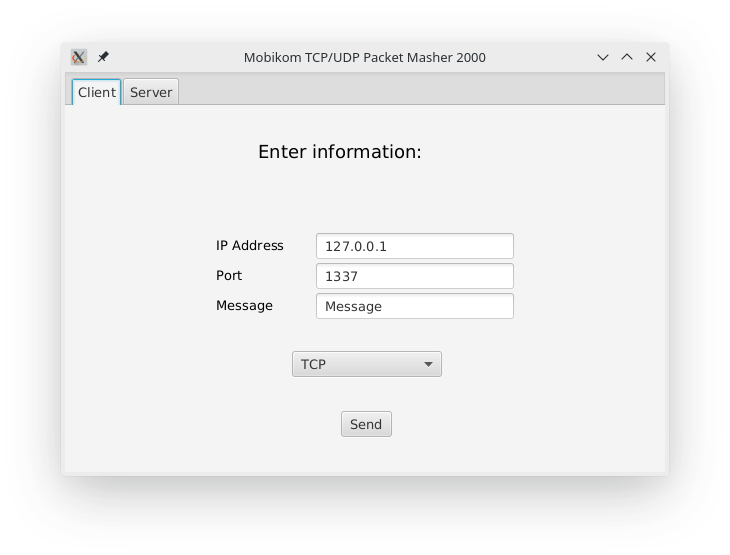
\includegraphics[width=1\linewidth]{images/task3/desktopTCP.png}
		\caption{The server interface with JavaFX}
		\label{fig:desktopTCP}
	\end{subfigure}
\begin{subfigure}{.49\textwidth}
	\centering
	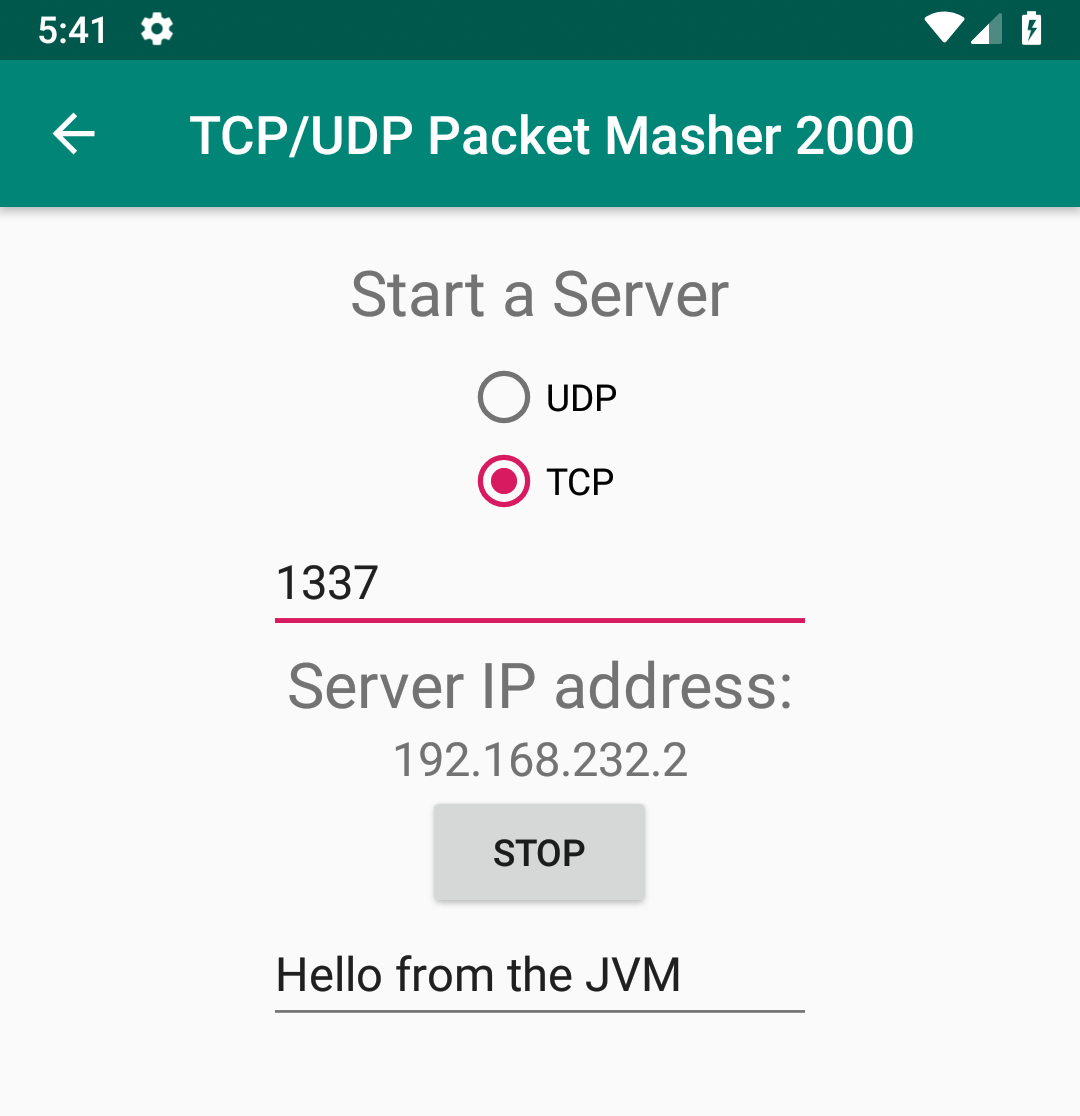
\includegraphics[width=0.74\linewidth]{images/task3/AndroidTCP.png}
	\caption{The client interface with JavaFX}
	\label{fig:androidTCP}
\end{subfigure}%
	\caption{Server in the Android emulator}
	\label{fig:emulator}
\end{figure}


\begin{figure}[H]
	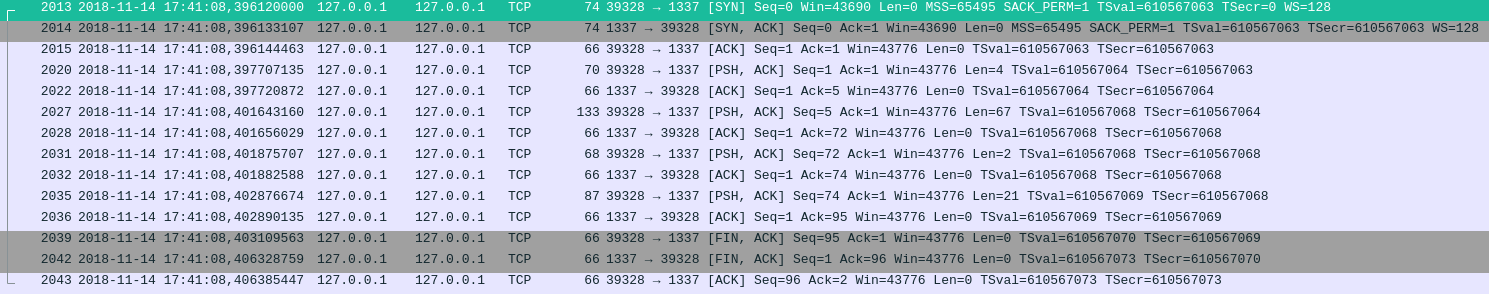
\includegraphics[width=1\linewidth]{images/task3/wiresharkAndroidEmuServer.png}
	\caption{Wireshark traces where Android App acts as a TCP server}
	\label{fig:wire1}
\end{figure}